\documentclass[12pt]{article}
\usepackage[left=2cm,right=2cm,top=2cm,bottom=2cm,bindingoffset=0cm]{geometry}
\usepackage[utf8x]{inputenc}
\usepackage[russian]{babel}
\usepackage{amsmath}
\usepackage{graphicx}
\usepackage{hyperref}

\graphicspath{ {./images/} }

\title{Задача оптимизации расписания с использованием алгоритма имитации отжига}
\author{Забровский Валерий Владимирович}
\date{Вариант 1}

\begin{document}
\maketitle

\section*{Формальная постановка задачи}

\subsection*{Дано}
\begin{itemize}
    \item множество независимых работ $W = \{W_i\}_{i=1}^{N}$;
    \item время выполнения $t_i$ работы $W_i$, $i = \overline{1, N}$;
    \item множество процессоров $P = \{p_i\}_{i=1}^{M}$.
\end{itemize}

\subsection*{Требуется}
Построить расписание выполнения работ $W$ на $M$ процессорах без прерываний так,
что достигается минимум критерия~\hyperref[crit]{$K_1$}.

\subsection*{Расписание}

Введём булеву матрицу $S \in \{0, 1\}^{M \times N}$,
где $S_{ij} = 1$, если на процессоре $p_i$ выполняется работа $W_j$,
и $S_{ij} = 0$ иначе.

Для каждого процессора $p_i$, $i = \overline{1, M}$, введём множество
всех работ, определённых на выполнение на данном процессоре:
\begin{equation}
    \Pi_i = \bigcup\limits_{\substack{j=1 \\ S_{ij}=1}}^N \{W_j\}.
\end{equation}
При этом $\bigcup\limits_{i=1}^M \Pi_i = W$.

Каждое множество $\Pi_i$, $i = \overline{1, M}$, упорядочим по невозрастанию
длительности работ, входящих во множество:
\begin{equation}
    \Pi_i = \{W_{i_k}\}_{k=1}^{|\Pi_i|},~
    t_{i_1} \geq t_{i_2} \geq \dots \geq t_{i_{|\Pi_i|}}.
\end{equation}

Для каждой работы $W_j$, $j = \overline{1, N}$, обозначим время начала и конца
выполнения через $T_B(W_j)$ и $T_E(W_j)$ соответственно.
При этом $0 \leq T_B(W_j) \leq T_E(W_j)$.

С учётом введённого выше порядка на множествах $\Pi_i$, $i = \overline{1, M}$,
для $\forall W_{i_s} \in \Pi_i$,
$i = \overline{1, M}$, $s = \overline{1, |\Pi_i|}$, справедливо
\begin{equation}
    T_E(W_{i_s}) = \sum\limits_{k=1}^s (\varepsilon_{i_k} + t_{i_k}),
\end{equation}
\begin{equation}
    T_B(W_{i_{s + 1}}) = T_E(W_{i_s}) + \overline\varepsilon_{i_{s+1}}~
    (s \neq |\Pi_i|),
\end{equation}
\begin{equation}
    T_B(W_{i_1}) = \overline\varepsilon_{i_1},
\end{equation}
$\varepsilon_k \geq 0, \overline\varepsilon_k \geq 0$.

Итак, расписание задаётся множествами $\Pi_i$, $i = \overline{1, M}$,
с введённым на них порядком.

\subsection*{Минимизируемый критерий}
\label{crit}
Разбалансированность расписания
\begin{equation}
    K_1 = T_{\max} - T_{\min},
\end{equation}
\begin{equation}
    T_{\max} = \max_{j = \overline{1, N}} T_E(W_j),
\end{equation}
\begin{equation}
    T_{\min} = \min_{j = \overline{1, N}} T_E(W_j).
\end{equation}

\subsection*{Ограничения}
Каждая работа $W_j$, $\forall j = \overline{1, N}$:
\begin{itemize}
    \item выполняется без прерываний и задержек:
    $\forall i~\varepsilon_i = \overline\varepsilon_i = 0$, т.е.
    \begin{equation}
        T_E(W_j) = T_B(W_j) + t_j
    \end{equation}
    и
    \begin{equation}
        \forall \Pi_i~T_B(W_{i_1}) = 0;
    \end{equation}

    \item выполняется строго на одном процессоре, т.е.
    $\exists! \Pi_i:~W_j \in \Pi_i;$

    \item имеет фиксированное время выполнения: $t_j = \text{const}$.
\end{itemize}

\section{Исследование последовательной реализации}

Рассматривались следующие законы понижения температуры:
\begin{itemize}
    \item Больцмана: $T = \frac{T_0}{\ln(1+i)}$;
    \item Коши: $T = \frac{T_0}{1+i}$;
    \item <<смешанный>>: $T = T_0\frac{\ln(1+i)}{1+i}$,
\end{itemize}
где $T_0$~-- начальная температура, $i$~-- номер итерации.

Для исследования генерировались случайные наборы работ с длительностями
от 1 до 128 у.е. Наборы имели размеры от 128 до 4096 работ и размещались на
количестве процессоров от 2 до 10. Для каждого набора алгоритм был запущен
5 раз. Среднее время работы отражено на рис.~1.

\begin{figure}[!h]
    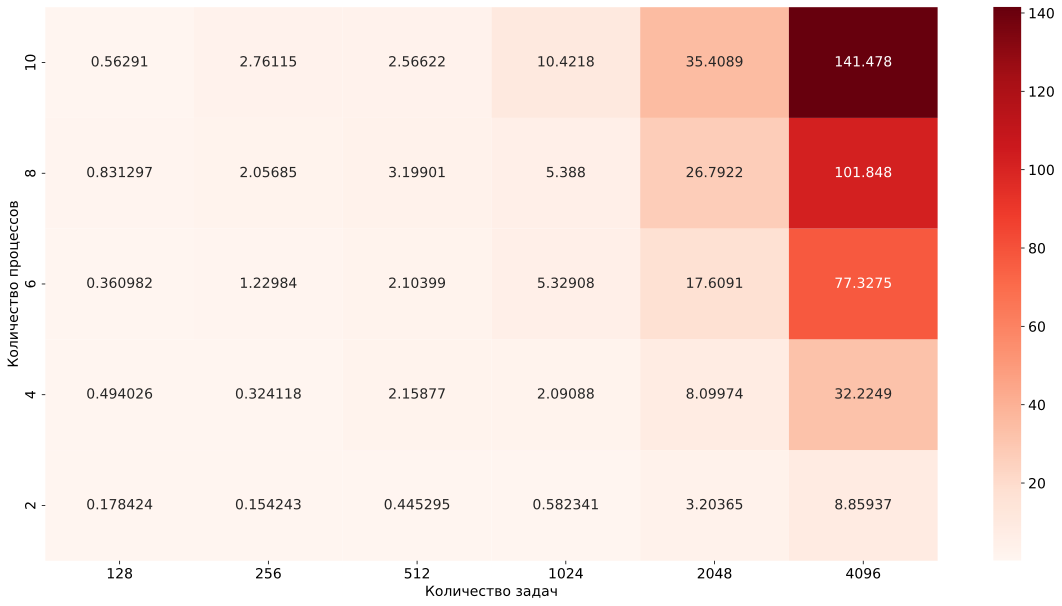
\includegraphics[width=\textwidth,keepaspectratio]{heatmap.png}
    \caption{Результаты исследования на примере закона Коши}
\end{figure}

Карта показывает, что время работы увеличивается с ростом числа процессоров
и с ростом количества работ. Наиболее продолжительным по времени работы
оказался алгоритм с законом Больцмана, при этом в большинстве случаев его
результаты были менее точными, нежели у алгоритма с законом Коши.
Алгоритм со <<смешанным>> законом работал несколько дольше, чем алгоритм
с законом Коши, однако их точность оказалась сопоставимой.

\section{Исследование параллельной реализации}

Для исследования был сформирован случайный набор 2048 работ с длительностями
от 1 до 128 у.е. для 8 процессоров. Алгоритм был запущен с законом Коши
по 10 раз на 1, 2, 4 и 8 потоках. Среднее время и качество отражены на рис.~2.

\begin{figure}[!h]
    \centering
    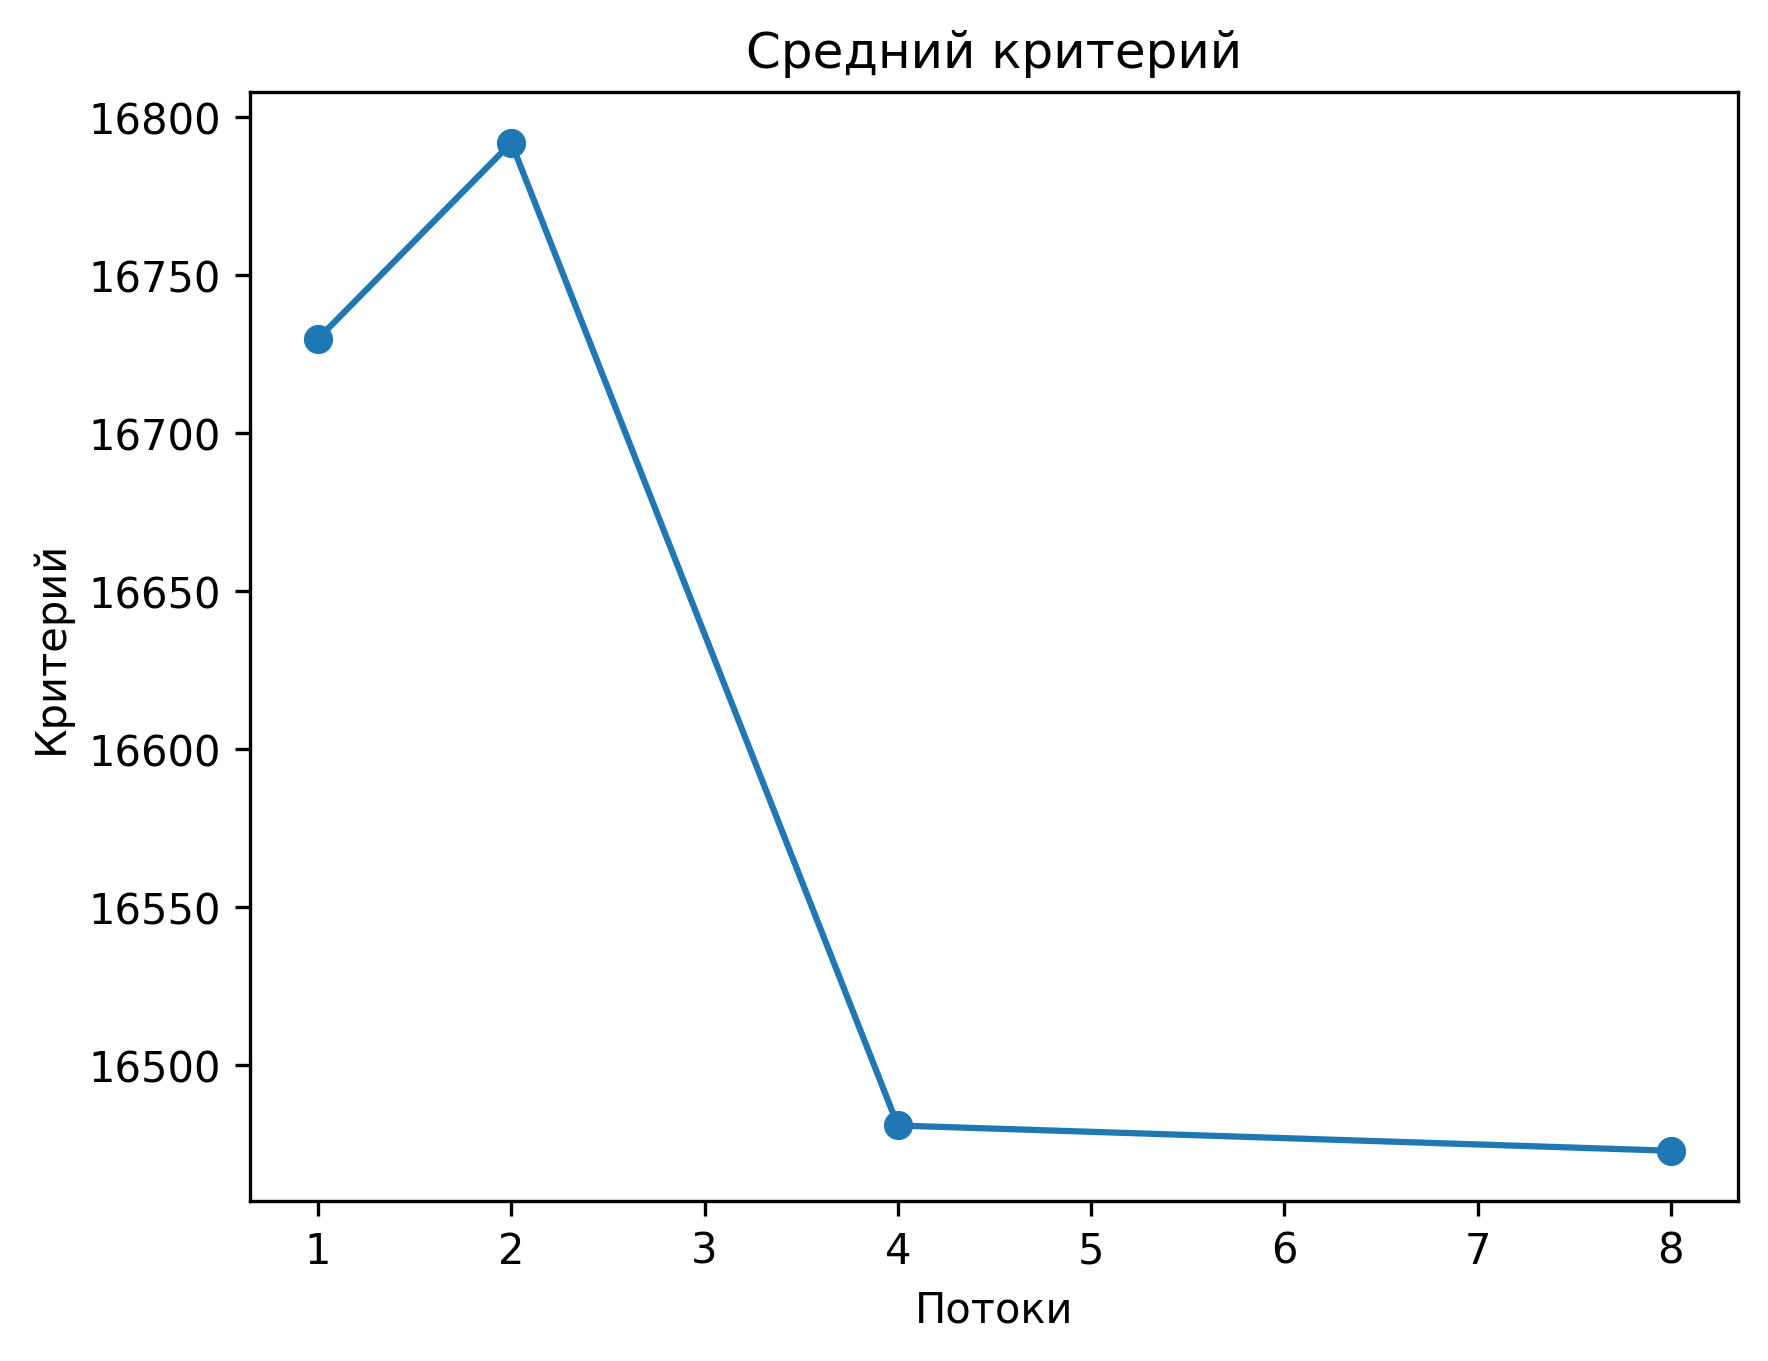
\includegraphics[width=0.45\textwidth,keepaspectratio]{criterion.png}
    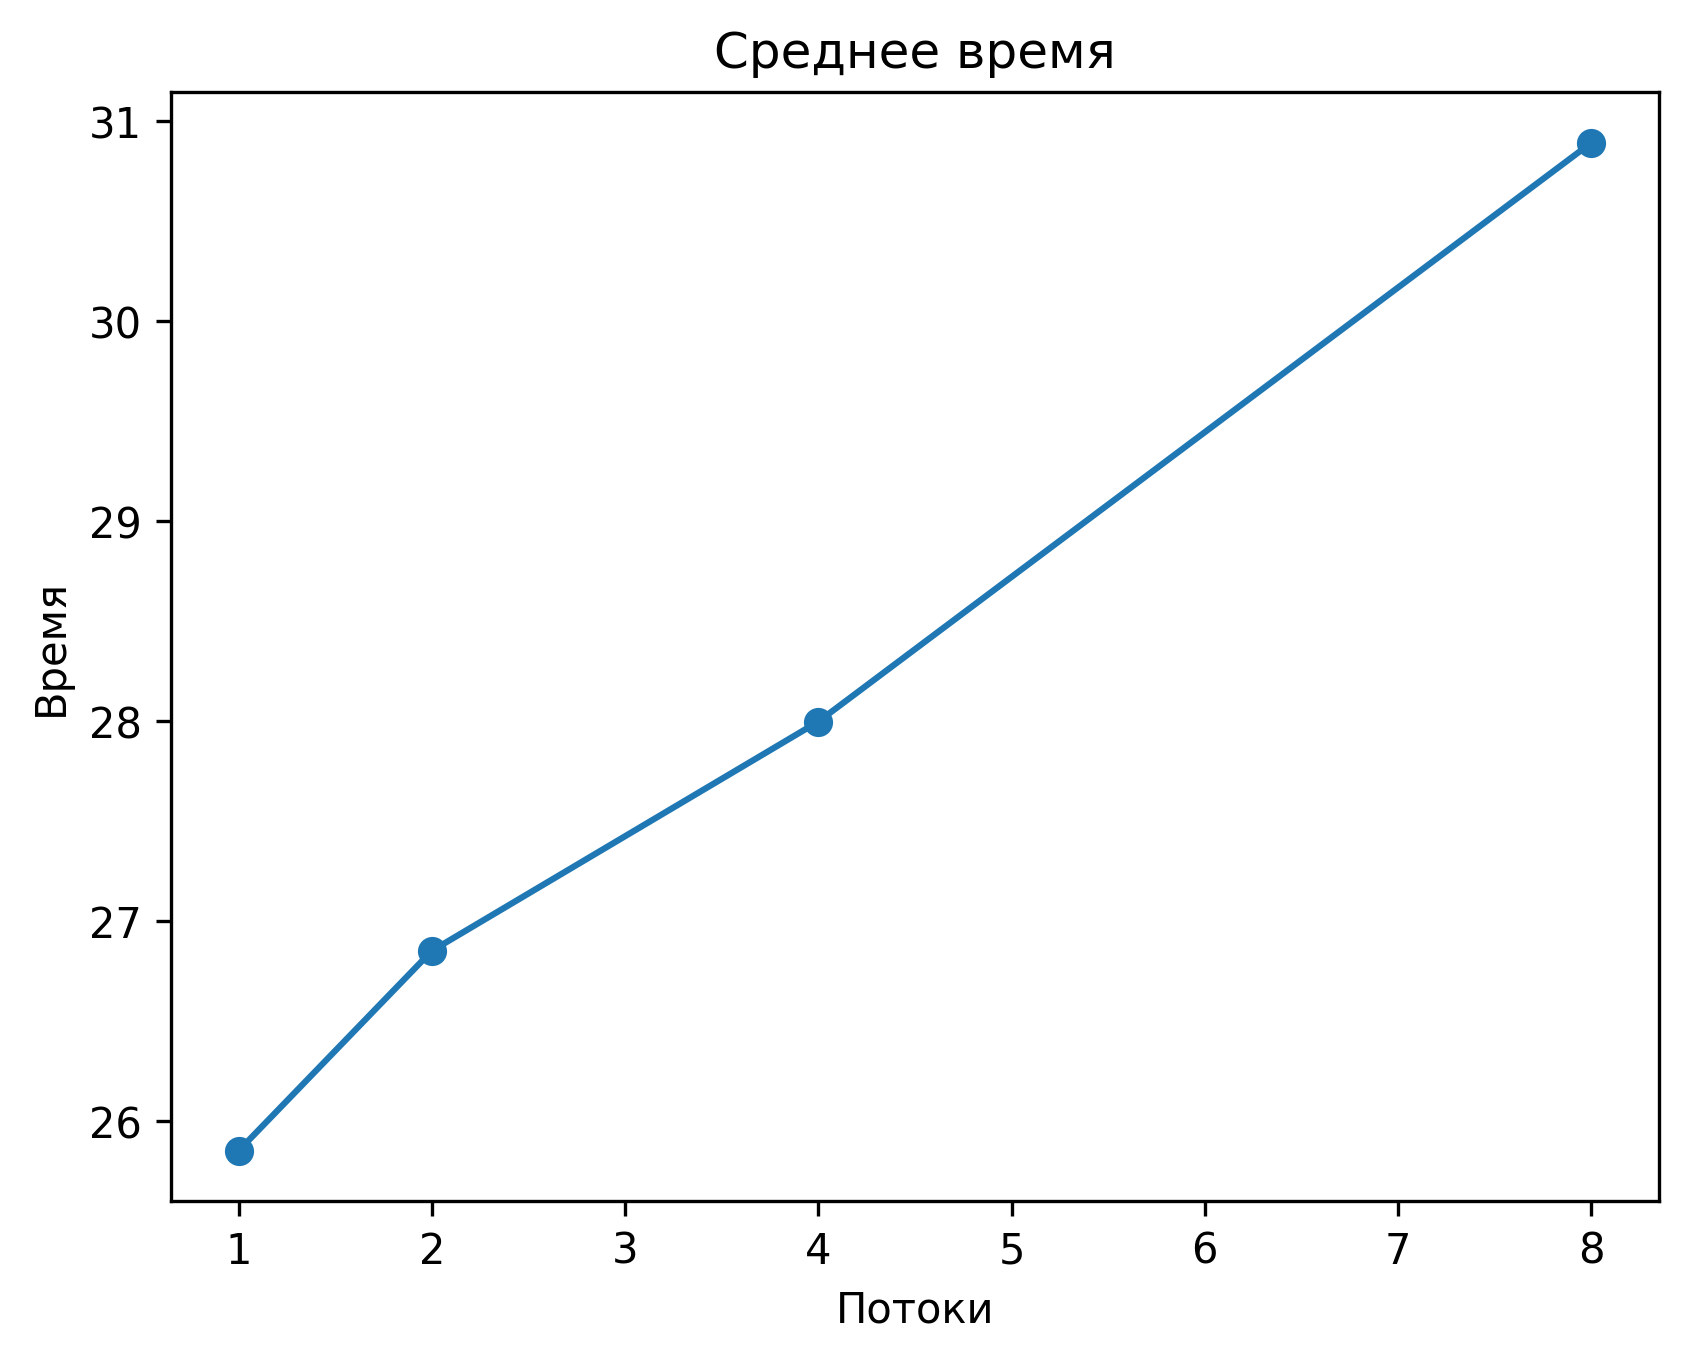
\includegraphics[width=0.45\textwidth,keepaspectratio]{time.png}
    \caption{Результаты исследования}
\end{figure}

Графики показывают, что время работы почти неизменно, однако точность
возрастает с увеличением количества потоков. Поэтому параллельная реализация
предпочтительнее последовательной.

\end{document}
